\section{RESEARCH RESULTS}

\begin{figure*}[h]
  \centering
  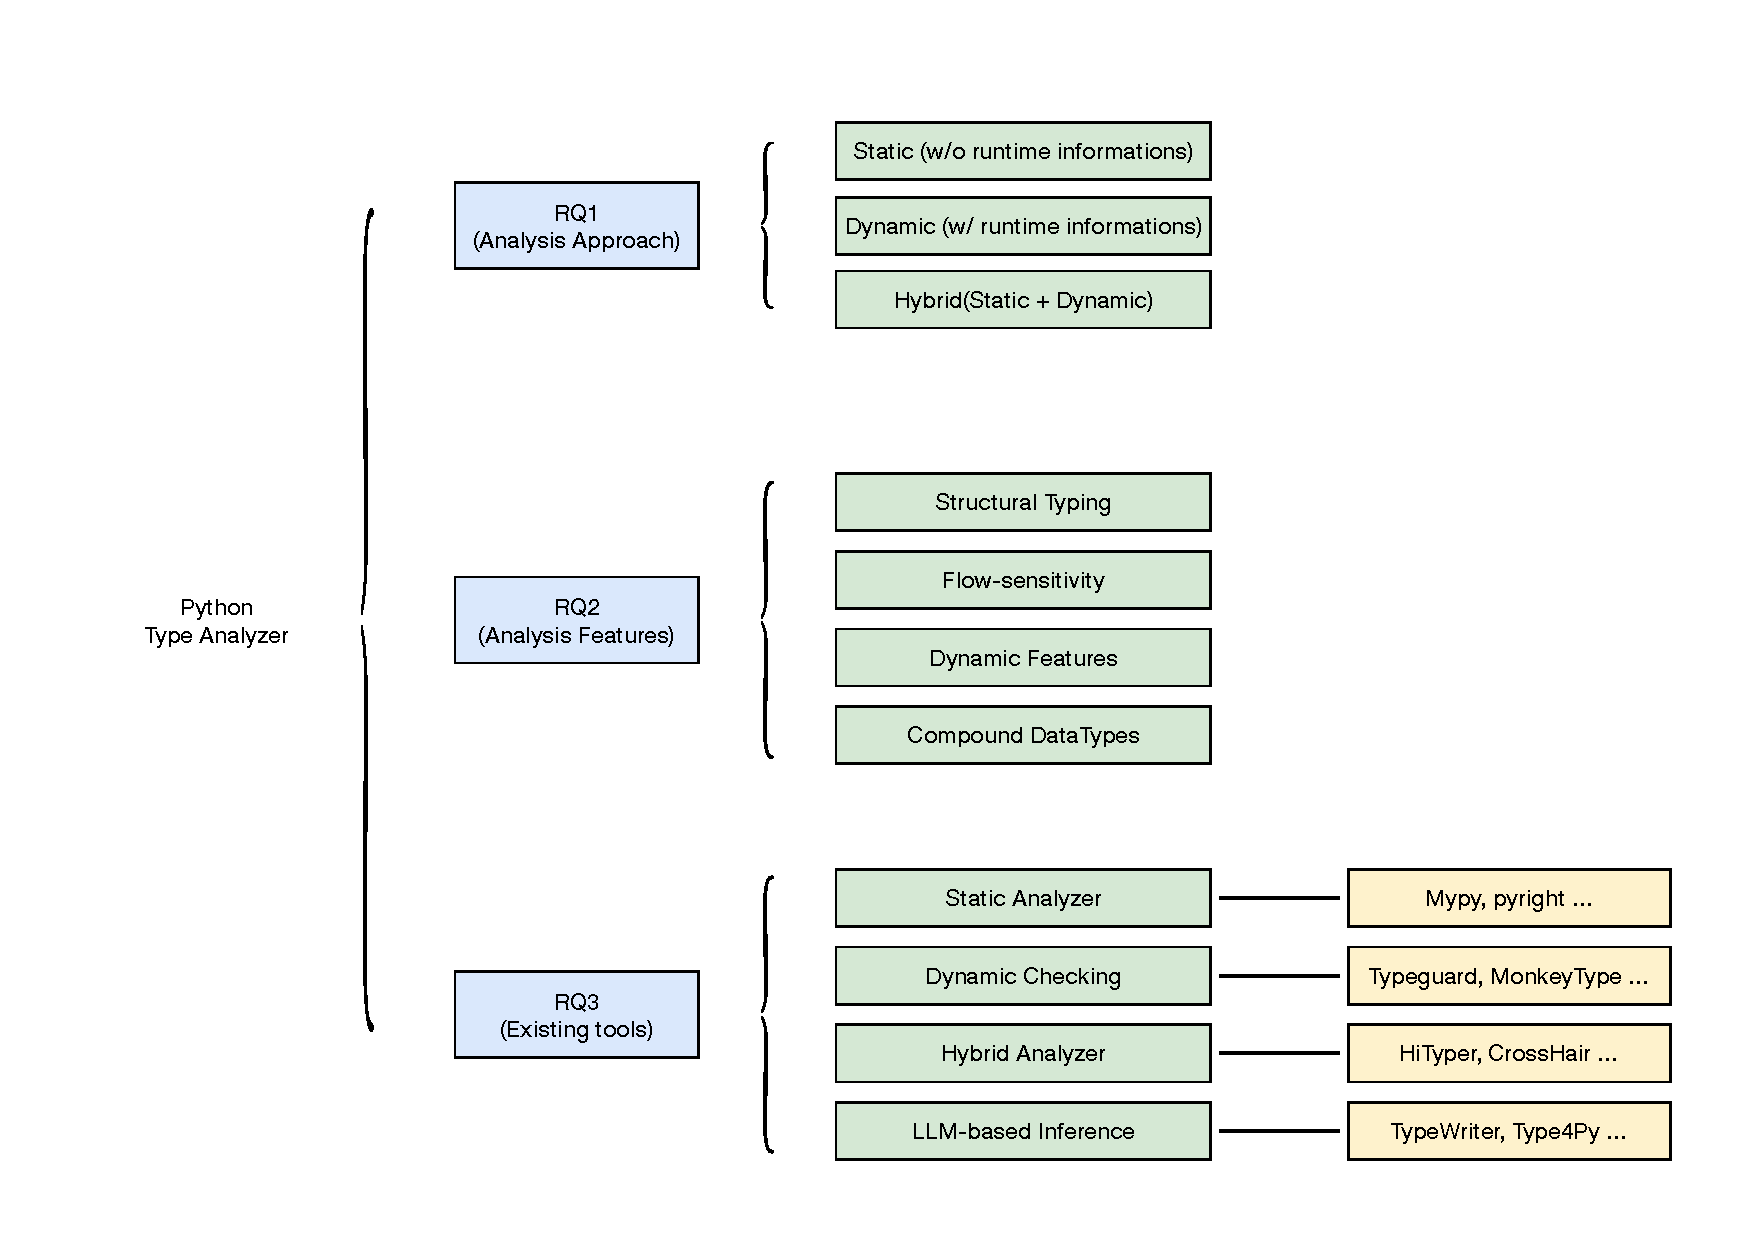
\includegraphics[width=\textwidth]{figures/overview2.pdf}
  \caption{Overview of Python type analysis in relation to the research questions (RQ1–RQ3).}
  \label{fig:rq_overview}
\end{figure*}

In this paper, we aim to provide a comprehensive understanding of how Python
type analysis has evolved and what technical strategies underpin current
approaches.
To this end, we systematically classify the major type analysis techniques used
in Python, as illustrated in \autoref{fig:rq_overview}, and compare their
technical characteristics, strengths, weaknesses, and representative tools.
Through this structured examination, we clarify the design trade-offs embedded
in each approach, identify the fundamental limitations shared across existing
techniques, and outline promising future research directions to address these
challenges.

\subsection{\textbf{Select Papers}}
In this survey, we aim to provide a comprehensive review of research on Python
type analysis and type checking. To identify relevant studies, we conducted a
systematic search of the literature using keywords such as “type analysis,”
“static type checking,” and “dynamic type checking.” From the retrieved
studies, we selected only those that focus on Python or explicitly address the
dynamic characteristics of Python programs in their type inference or type
checking techniques.

Based on these criteria, the survey includes traditional static type
analyses~\cite{static2014}, constraint-based approaches~\cite{MaxSMT2018},
machine learning–driven methods~\cite{pyinfer2021,lambdanet2020,typeT52023},
and hybrid techniques combining static analysis and
learning~\cite{hityper2022,static2023,dlinfer2023}. 
In addition, we also consider studies that aim to predict or repair Python
runtime type errors~\cite{pyter2022,pyty2024,pyinder2024,quac2024}, covering
research that extends beyond pure type inference to practical program
improvement.

The selected studies collectively address diverse aspects of Python type
analysis, including handling dynamic features, compound data types, and flow
sensitivity. They represent a broad spectrum of methodologies—static, dynamic,
and learning-based approaches—and are thus well-suited for a comprehensive
comparison and discussion of the current state and future directions of Python
type checking research.

\subsection{\textbf{RQ1 : How can Python’s dynamic nature be preserved while ensuring
  program stability through type checking?}}

Because Python is a dynamically typed language, the actual structure and state
of objects are determined only at runtime.
While this design provides significant flexibility and expressiveness for
developers, it inevitably reduces the precision attainable through static
analysis and increases the likelihood of runtime errors such as TypeError and
AttributeError.
As a result, the research community has proposed a wide range of analysis
techniques that attempt to improve program reliability while still preserving
Python’s dynamic nature.
These approaches vary widely in their assumptions, goals, and underlying
technical mechanisms—from purely static inference to hybrid and
runtime-assisted analyses—reflecting the difficulty of balancing soundness,
precision, and usability in such a dynamic environment.

\autoref{tab:RQ1} summarizes the number of existing type checking approaches,
providing an overview of the landscape. The following sections examine each
category in detail and analyze their strengthes and limitations.


\begin{table}[ht]
  \centering
  \caption{Number of papers and tools classified by Type Checking Approaches (RQ1).}
  \label{tab:RQ1}
  \small
  \setlength{\tabcolsep}{3pt} % 좌우 여백 축소
  \begin{tabularx}{\columnwidth}{
    >{\centering\arraybackslash}X|
    >{\centering\arraybackslash}X|
    >{\centering\arraybackslash}X}
    \toprule
    \textbf{Static} & \textbf{Dynamic} & \textbf{Hybrid} \\
    \midrule
    \multicolumn{1}{>{\centering\arraybackslash}X|}{21} &
    \multicolumn{1}{>{\centering\arraybackslash}X|}{2} &
    \multicolumn{1}{>{\centering\arraybackslash}X}{4} \\
    \bottomrule
  \end{tabularx}
\end{table}


\subsubsection{\textbf{Static Type Checking with Type Annotations}}


Since the introduction of type annotations, it has become possible to enhance
program reliability using explicit static type information.
Static type checkers such as Mypy~\cite{mypy} and Pyre~\cite{pyre} were
developed on this basis, enabling the detection of potential TypeError in
variables, function parameters, and return values before execution.
Moreover, Python adopts a gradual typing approach, allowing static verification
even when only parts of a program are annotated.
This enables developers to strengthen type safety incrementally.
Typically, static type checking verifies, as in
Algorithm~\autoref{alg:gradualtyping}, whether the code matches the provided
type annotations and may further perform type inference to ensure correct use
of types in practice.

\autoref{tab:RQ1} shows that static approaches constitute the largest portion
of existing research and tools.
This prevalence can be attributed to two factors.
First, static type checking imposes no runtime overhead, making it attractive
for industrial use where performance is critical.
Second, type annotation support in Python has steadily matured—particularly
with the introduction of type hints (PEP 484), generics (PEP 585), and gradual
typing infrastructures—providing a well-defined foundation upon which many
tools have been developed.
As a result, static analysis has become the most accessible and practically
deployable method for improving Python’s reliability.

However, because static analysis is limited to annotated regions, it cannot
provide the same level of safety guarantees as fully statically typed
languages. Furthermore, Python’s type annotations rely primarily on nominal
typing, which limits their ability to accurately capture Python’s structural
and behavior-based typing semantics, such as duck typing based on the presence
of specific methods or attributes. Therefore, while static type checking has
the advantage of detecting errors in advance without incurring runtime
overhead, it suffers from a high rate of false positives due to its difficulty
in capturing Python’s dynamic behavior.

% -------------------------
\begin{algorithm}[t]
\caption{GradualTypeCheck}
\begin{algorithmic}[1]
\REQUIRE Python function $f$ with optional type annotations, arguments $args$
\ENSURE TypeError if type mismatch detected
\FOR{each argument $a_i$ in $args$}
    \IF{$f$ has type annotation for $a_i$}
        \IF{type($a_i$) $\neq$ annotation\_type($a_i$)}
            \STATE raise TypeError
        \ENDIF
    \ENDIF
\ENDFOR
\STATE result = execute($f$, $args$)
\IF{$f$ has return type annotation}
    \IF{type(result) $\neq$ annotation\_type($f$.return)}
        \STATE raise TypeError
    \ENDIF
\ENDIF
\STATE \textbf{return} result
\end{algorithmic}
\label{alg:gradualtyping}
\end{algorithm}
% -------------------------


\subsubsection{\textbf{Dynamic Monitering and Runtime Enforcement}}
Dynamic type monitoring and runtime enforcement observe type-related
constraints during the actual execution of a program and report violations
immediately.
Although this approach cannot capture all errors prior to execution—as static
analysis attempts to do—it provides high accuracy for type violations along
concrete execution paths.
In languages such as Python, where dynamic binding is pervasive, this approach
is particularly practical because it can directly reproduce behavior-based
runtime errors that static techniques often fail to detect.

The most widely used runtime enforcement mechanism is decorator-based wrapping.
By attaching a type-checking decorator to a function, as in
Algorithm~\autoref{alg:monitering}, the checker verifies at each call whether
the argument and return values conform to the declared type annotations.
Libraries such as typeguard~\cite{typeguard} implement this strategy using
typing.get\_type\_hints() and isinstance-based checks.
This method requires minimal modification to existing code and detects
mis-typed values precisely at the point of failure, making it highly effective
for debugging.
However, because checks are executed on every function call, runtime overhead
is unavoidable, and complex type structures—such as generics, nested container
types—cannot always be validated at runtime.

Another form of dynamic monitoring leverages runtime traces for downstream
analyses.
MonkeyType~\cite{monkeytype}, for example, records observed argument and return
types during test execution and automatically generates Mypy-compatible
annotations.
Because this approach captures real execution behavior, it is particularly
useful for inferring types in legacy systems or analyzing complex functions.
Nevertheless, it critically depends on test quality and coverage; types for
rarely executed paths or untested branches remain unknown.

Dynamic enforcement therefore provides high precision on observed paths but
suffers from fundamental limitations.
Achieving comprehensive program safety requires sufficiently broad test or
execution coverage, creating substantial coverage dependency and potentially
high execution cost.
Furthermore, runtime information alone is often insufficient to accurately
validate deeply nested or generic types, protocol-based structural constraints,
or types involving implicit invariants.
Techniques such as conditional checks, sampling-based monitoring, or partial
instrumentation can mitigate overhead, but they cannot fully eliminate these
inherent weaknesses.

In practice, Python’s dynamic analysis ecosystem reflects these trade-offs.
typeguard offers decorator-based runtime checking, MonkeyType synthesizes
annotations from runtime traces, and CrossHair~\cite{crosshair} combines
dynamic execution with symbolic reasoning for hybrid verification. 
Collectively, these tools complement static checkers by addressing classes of
errors that remain challenging to detect in a highly dynamic language such as
Python.

% -------------------------
\begin{algorithm}[H]
\caption{RuntimeTypeMonitor}
\begin{algorithmic}[1]
\REQUIRE Python function $f$ with optional type annotations
\ENSURE Detect type violations during execution
\STATE Wrap $f$ with a type-checking decorator
\STATE On each call to $f$:
\FOR{each argument $a_i$}
    \IF{type annotation exists for $a_i$}
        \IF{type($a_i$) $\neq$ annotation\_type($a_i$)}
            \STATE Log type violation
        \ENDIF
    \ENDIF
\ENDFOR
\STATE Execute original function $f$
\IF{return type annotation exists}
    \IF{type(return) $\neq$ annotation\_type(return)}
        \STATE Log type violation
    \ENDIF
\ENDIF
\end{algorithmic}
\label{alg:monitering}
\end{algorithm}
% -------------------------


\subsubsection{\textbf{Hybrid Approaches}}
To address both Python’s dynamic nature and the inherent limitations of static
analysis, recent research has increasingly focused on hybrid analysis, which
integrates static and dynamic techniques into a unified framework.
By combining the global reasoning power of static analysis with the
execution-based precision of dynamic monitoring, hybrid methods aim to provide
more practical and robust guarantees for Python programs.

A familiar instance of such integration is the combination of gradual typing
with runtime checking.
Tools such as Mypy and Pyre statically verify annotated code regions while
validating unannotated or ambiguous segments at runtime, thereby reducing
static false positives and improving overall reliability.
Nevertheless, these approaches are not counted as hybrid in \autoref{tab:RQ1},
because they rely primarily on annotation-driven static checks combined with
simple runtime guards, rather than incorporating substantial runtime
information into the analysis process.

In \autoref{tab:RQ1}, hybrid approaches refer specifically to techniques that
use both compile-time and runtime information as essential components of the
analysis.
Examples include methods that enrich static constraints using execution traces,
that integrate dynamic attribute access patterns into static reasoning, or that
iteratively refine abstractions using runtime-observed types.
Likewise, analyses that combine symbolic reasoning with concrete execution fall
within this category.
Conversely, AI-based techniques trained solely on static code features are
excluded because they utilize only compile-time information.

By leveraging dynamic observations to refine or correct the conservatism of
static analysis, hybrid methods can reflect Python’s real-world usage patterns
more faithfully and significantly reduce spurious warnings.
At the same time, static analysis provides a global viewpoint that compensates
for the path-specific nature of dynamic monitoring, enabling broader safety
guarantees that cannot be achieved by runtime techniques alone.
This combination often yields higher type safety, improved precision, and
greater tool usability than either approach by itself.

However, hybrid methods also inherit several challenges.
Because they depend on runtime information, their effectiveness is tied to the
availability and coverage of executed paths; insufficient execution data can
limit their precision.
Runtime monitoring and trace collection introduce performance overhead, and the
integration of static and dynamic information imposes additional computational
and engineering costs. Despite these limitations, hybrid analysis remains one
of the most promising research directions for Python type analysis, offering a
balanced and practical means of handling the language’s highly dynamic
semantics.

\subsubsection{\textbf{Summary: Landscape of Type Analysis Techniques for Python}}
Because Python is fundamentally a dynamically typed language, fully static type
checking—of the kind possible in statically typed languages—is structurally
infeasible.
Object attributes may be added, removed, or modified at runtime, and even the
return type of a single function may vary depending on control flow.
Despite these challenges, recent advances in type analysis have demonstrated
that Python can achieve a meaningful degree of type safety through a
combination of complementary techniques.

As discussed in the previous sections, existing approaches fall into three
major directions, each with distinct strengths and limitations.
First, annotation-based static analysis performs ahead-of-time verification and
can detect errors early without incurring runtime costs.
Its global reasoning capability allows broad safety guarantees. However, its
inherent conservatism and difficulty in modeling Python’s dynamic behavior
often lead to false positives, particularly in unannotated or highly dynamic
regions.
Second, runtime monitoring and enforcement provide high precision for observed
execution paths and faithfully capture dynamic semantics that static methods
miss.
Yet these techniques depend heavily on execution coverage, introduce runtime
overhead, and cannot ensure global safety unless extensive tests or traces are
available.
Third, hybrid approaches integrate static and dynamic information, allowing
static analysis to be refined using concrete runtime observations.
This reduces false positives, increases practical precision, and better
reflects real-world usage patterns. At the same time, hybrid analysis still
inherits certain limitations—such as coverage dependence and the cost of
merging diverse information sources—but offers a balanced compromise between
static safety and dynamic flexibility.

In summary, while no single technique can provide complete type safety for
Python, these three categories collectively define the current landscape of
Python type analysis.
Among them, hybrid approaches are gaining prominence, as they leverage the
complementary strengths of static reasoning and dynamic evidence to address
Python’s dynamic nature more effectively than either method alone.

\begin{tcolorbox}[colback=white,colframe=blue!60,title=Answer to RQ1,fonttitle=\bfseries]
  Recent work shows a clear shift from purely static analysis toward hybrid and
  runtime-assisted approaches for Python type checking. Static analyzers still
  play a central role in large-scale verification, but runtime monitoring
  complements them by capturing behaviors that static methods miss. As a
  result, hybrid systems have become the most practical way to balance Python’s
  dynamic nature with meaningful type safety.
\end{tcolorbox}

\subsection{\textbf{RQ2 : What are the main challenges in type inference and
  type analysis for Python programs?}}

\begin{table*}[ht]
\centering
\small
\setlength{\tabcolsep}{4pt} % 열 간격 조정
\caption{RQ2: Table showing whether existing Python type analysis papers and
  tools support key Python features, including structural typing,
  flow-sensitive types, dynamic features, and compound data types.
  (\cmark~ is support, \xmark~ is not.)}
  \begin{tabularx}{\textwidth}{>{\centering\arraybackslash}X
                               >{\centering\arraybackslash}X
                               >{\centering\arraybackslash}X
                               >{\centering\arraybackslash}X
                               >{\centering\arraybackslash}X}
  \toprule
  \rowcolor{yellow!30}
  \textbf{Paper/Tool} & \textbf{Structural Typing} & \textbf{Flow-sensitivity} & \textbf{Dynamic Features} & \textbf{Compound DataTypes} \\
  \midrule
    \rowcolor{green!10} \cite{static2014} & \xmark & \xmark & \xmark & \cmark \\
    \rowcolor{white} \cite{static2015} & \xmark & \xmark & \xmark & \cmark \\
    \rowcolor{green!10} \cite{MaxSMT2018} & \xmark & \cmark & \xmark & \cmark \\
    \rowcolor{white} \cite{prob2016} & \xmark & \xmark & \cmark & \cmark \\
    \rowcolor{green!10} \cite{DL2018} & \xmark & \xmark & \cmark & \cmark \\
    \rowcolor{white} \cite{typewriter2020} & \xmark & \xmark & \cmark & \cmark \\
    \rowcolor{green!10} \cite{lambdanet2020} & \xmark & \xmark & \cmark & \cmark \\
    \rowcolor{white} \cite{pyter2022} & \xmark & \cmark & \cmark & \cmark \\
    \rowcolor{green!10} \cite{static2021} & \xmark & \cmark & \cmark & \cmark \\
    \rowcolor{white} \cite{hityper2022} & \xmark & \cmark & \cmark & \cmark \\
    \rowcolor{green!10} \cite{type4py2022} & \xmark & \xmark & \cmark & \cmark \\
    \rowcolor{white} \cite{pyinfer2021} & \xmark & \xmark & \cmark & \cmark \\
    \rowcolor{green!10} \cite{static2023} & \xmark & \xmark & \cmark & \cmark \\
    \rowcolor{white} \cite{pyty2024} & \xmark & \cmark & \cmark & \cmark \\
    \rowcolor{green!10} \cite{dlinfer2023} & \xmark & \cmark & \cmark & \cmark \\
    \rowcolor{white} \cite{tipical2023} & \xmark & \cmark & \xmark & \cmark \\
    \rowcolor{green!10} \cite{typeT52023} & \xmark & \xmark & \cmark & \cmark \\
    \rowcolor{white} \cite{pyinder2024} & \cmark & \cmark & \cmark & \cmark \\
    \rowcolor{green!10} \cite{quac2024} & \cmark & \cmark & \cmark & \cmark \\
    \rowcolor{white} \cite{monkeytype} & \xmark & \xmark & \cmark & \cmark \\
    \rowcolor{green!10} \cite{crosshair} & \xmark & \xmark & \cmark & \cmark \\
    \rowcolor{white} \cite{typeguard} & \xmark & \xmark & \cmark & \cmark \\
    \rowcolor{green!10} \cite{mopsa2020} & \cmark & \cmark & \cmark & \cmark \\
    \rowcolor{white} \cite{mypy} & \xmark & \xmark & \xmark & \cmark \\
    \rowcolor{green!10} \cite{pyre} & \xmark & \cmark & \cmark & \cmark \\
    \rowcolor{white} \cite{pytype} & \xmark & \cmark & \cmark & \cmark \\
    \rowcolor{green!10} \cite{pyright} & \xmark & \cmark & \cmark & \cmark \\
  \midrule
  \rowcolor{pink!30} 27 & 3 & 13 & 22 & 27 \\
  \bottomrule
  \end{tabularx}
  \label{tab:RQ2}
\end{table*}


Type analysis in Python is fundamentally more challenging than in traditional
statically typed languages due to its structural and dynamic characteristics.
In particular, (1) structural typing–based object compatibility, (2)
flow-sensitive types that change according to control flow, (3) advanced
dynamic features such as reflection and dynamic code generation, and (4) the
presence of heterogeneous containers are frequently cited as the primary
obstacles to precise type analysis.
\autoref{tab:RQ2} shows whether existing research and tools support these four key
Python features.
Each column corresponds to one of the four challenges, and the entries indicate
whether a particular paper or tool provides support.
This provides a clear overview of the strengths and limitations of current
Python type analysis approaches.

First, Python follows a duck-typing model that is closer to structural typing
than nominal typing. The meaning of an object is determined by the methods and
attributes it provides, making it difficult to accurately model objects using
only static type names. Most existing studies do not use structural typing;
instead, they perform analysis based solely on type names (nominal typing). For
this reason, current approaches cannot dynamically model Python’s types,
leading to high uncertainty in static type inference.

Second, the type of a Python variable may vary depending on the program’s
control flow. A single variable may assume different types across different
branches, making it difficult for traditional static analysis to infer a
consistent type. To address this, recent studies perform flow-sensitive
analysis, but only about 50\% of the works apply it; the rest rely on methods
derived from static-typed languages that do not account for control flow.
Flow-insensitive analysis sometimes uses techniques such as Static Single
Assignment (SSA) to represent control flow. However, increasing precision using
these methods rapidly raises computational costs. Therefore, flow-aware
analysis is essential, and balancing accuracy with performance remains a
central challenge in Python type analysis.

Third, Python’s powerful dynamic features—reflection and dynamic code
generation—fundamentally threaten the soundness of any static type analysis.
Dynamic attribute access via getattr and \_\_getattribute\_\_, runtime code
generation using eval() and exec(), dynamic module loading via importlib, and
metaclass-based class generation all defer program structure determination
until runtime. Accurately analyzing these features would require nearly full
program execution, making precise static type inference difficult within
traditional frameworks. However, as shown in \autoref{tab:RQ2}, about 80\% of studies
support some dynamic features; this is a generous count that includes partial
support. Full support for all dynamic features is not achievable in static
analysis except through execution-based approaches.

Finally, Python’s lists, sets, and dictionaries inherently allow heterogeneous
elements. A single list may contain integers, strings, and user-defined
objects, and element types may evolve during execution. Simple uniform type
models are insufficient, and more sophisticated representations—such as union
types, intersection types, or lattice-based type spaces—are required. All
surveyed studies and tools account for this feature, highlighting that
heterogeneous containers are a critically important aspect of Python type
analysis.

\begin{tcolorbox}[colback=white,colframe=blue!60,title=Answer to RQ2,fonttitle=\bfseries]
  Python type analysis exhibits high complexity due to
  (1) structural typing–based non-uniformity,
  (2) types that change continually depending on control flow,
  (3) the possibility of runtime code generation, and
  (4) heterogeneous containers.
  These characteristics make it difficult for traditional static analysis
  frameworks to achieve accurate and sound modeling, highlighting the need for
  new analysis paradigms tailored to Python’s inherently dynamic nature.
\end{tcolorbox}

\subsection{\textbf{RQ3 : What technical characteristics and limitations define
  existing Python type analysis tools?}}

The Python ecosystem includes a wide range of type analysis tools, spanning
static, dynamic, hybrid, and, more recently, LLM-based approaches.
Each category adopts a distinct technical strategy to handle Python’s highly
dynamic language characteristics, resulting in a mix of complementary strengths
and inherent limitations.
This section classifies major tools into four categories and analyzes their
technical features and constraints.

Static type checkers such as Mypy, Pyright, and Pyre are the most widely used
tools in practice.
These systems construct a type environment primarily from user-provided type
annotations and verify type consistency through constraint solving.
They support advanced features of Python’s typing system—such as Protocols and
TypedDicts—to enable structural subtyping, and they also provide partial type
inference.
This design yields fast analysis performance and reasonable precision for
large-scale codebases, making static analysis highly practical.
However, their heavy reliance on annotations means that accuracy degrades
sharply in real-world industrial code, where annotations are often missing or
incomplete.
Moreover, they cannot fully soundly model Python’s dynamic features such as
reflection, monkey patching, and dynamic attribute creation, resulting in
unavoidable false positives and false negatives.
In short, static analysis is “fast and practical but fundamentally incomplete.”

In contrast, dynamic and hybrid analysis tools leverage runtime information to
achieve higher accuracy.
Tools such as Typeguard and contract-based libraries validate arguments, return
values, and structural properties of objects at execution time, allowing them
to detect type violations soundly during actual program runs.
Tools like MonkeyType collect type hints from execution traces, enabling
high-precision, test-driven type inference.
These approaches require little to no annotation and can recover detailed type
information with high accuracy.
However, they structurally depend on test coverage: unexecuted paths cannot be
analyzed, which becomes a critical limitation given Python’s diverse dynamic
behaviors.
Runtime instrumentation also introduces performance overhead, limiting
applicability in large-scale or latency-sensitive systems.

Recent academic work explores more advanced static techniques, including
constraint-based analysis, symbolic execution, and SSA-based type analysis.
These approaches employ refined type models such as union-type lattices,
intersection types, and path-sensitive constraint solving to achieve higher
precision.
Symbolic execution allows simultaneous exploration of multiple execution paths,
mitigating the limited coverage of traditional static analysis, while SSA-based
approaches more accurately capture flow-sensitive type changes.
However, these techniques are computationally expensive and difficult to apply
to real-world codebases, especially in the presence of Python’s irregular
dynamic features such as eval, dynamic imports, and metaclasses. Scaling issues
(e.g., parameter explosion) further limit their practical deployment.

Finally, LLM-based type analysis—using models like GPT or CodeLlama—has
recently emerged as a new direction.
LLMs can infer types with high coverage even for codebases with minimal
annotations, and they can perform semantic-level reasoning by leveraging
natural-language context and code meaning.
This enables the detection of semantic type errors (e.g., API misuse, violation
of implicit assumptions) that traditional static analyzers often miss.
However, LLMs operate as black-box models; their reasoning processes are
opaque, subject to hallucination, and fundamentally unable to guarantee
soundness.
Their outputs are non-deterministic, making formal safety properties and
reproducibility—central requirements for static analysis—difficult to achieve.

In summary, Python type analysis tools exhibit complementary strengths
depending on their underlying analysis paradigm, but no single approach can
fully capture the complexity of Python’s dynamic semantics.
Static analysis is efficient yet incomplete, dynamic analysis is precise yet
coverage- and cost-constrained, and AI-based methods are flexible but lack
soundness.
Consequently, recent research trends increasingly favor hybrid approaches that
combine static, dynamic, and AI-based techniques.
This observation underscores that Python type analysis is not a problem
solvable by any single method.

\begin{tcolorbox}[colback=white,colframe=blue!60,title=Answer to RQ3,fonttitle=\bfseries]
  Python type analysis tools can be classified into static, dynamic,
  research-oriented, and LLM-based approaches. Static analysis is fast but
  struggles with dynamic features, while dynamic and hybrid methods offer
  accuracy at the cost of coverage and runtime overhead. LLM-based approaches
  enable semantic-level reasoning but lack determinism and soundness. Overall,
  no single technique is sufficient, and hybrid combinations of static, dynamic,
  and AI-based methods are becoming increasingly important.
\end{tcolorbox}

